%!TeX root=../wowtop.tex

\ArtChapter[The Exodus from London]{16head}



\lettrine[lines=4,findent=2pt]{S}{o} you understand the roaring wave of fear that swept through the greatest city in the world just as Monday was dawning—the stream of flight rising swiftly to a torrent, lashing in a foaming tumult round the railway stations, banked up into a horrible struggle about the shipping in the Thames, and hurrying by every available channel northward and eastward. By ten o'clock the police organisation, and by midday even the railway organisations, were losing coherency, losing shape and efficiency, guttering, softening, running at last in that swift liquefaction of the social body.

All the railway lines north of the Thames and the South-Eastern people at Cannon Street had been warned by midnight on Sunday, and trains were being filled. People were fighting savagely for standing-room in the carriages even at two o'clock. By three, people were being trampled and crushed even in Bishopsgate Street, a couple of hundred yards or more from Liverpool Street station; revolvers were fired, people stabbed, and the policemen who had been sent to direct the traffic, exhausted and infuriated, were breaking the heads of the people they were called out to protect.

And as the day advanced and the engine drivers and stokers refused to return to London, the pressure of the flight drove the people in an ever-thickening multitude away from the stations and along the northward-running roads. By midday a Martian had been seen at Barnes, and a cloud of slowly sinking black vapour drove along the Thames and across the flats of Lambeth, cutting off all escape over the bridges in its sluggish advance. Another bank drove over Ealing, and surrounded a little island of survivors on Castle Hill, alive, but unable to escape.

After a fruitless struggle to get aboard a North-Western train at Chalk Farm—the engines of the trains that had loaded in the goods yard there \textit{ploughed} through shrieking people, and a dozen stalwart men fought to keep the crowd from crushing the driver against his furnace—my brother emerged upon the Chalk Farm road, dodged across through a hurrying swarm of vehicles, and had the luck to be foremost in the sack of a cycle shop. The front tire of the machine he got was punctured in dragging it through the window, but he got up and off, notwithstanding, with no further injury than a cut wrist. The steep foot of Haverstock Hill was impassable owing to several overturned horses, and my brother struck into Belsize Road.

So he got out of the fury of the panic, and, skirting the Edgware Road, reached Edgware about seven, fasting and wearied, but well ahead of the crowd. Along the road people were standing in the roadway, curious, wondering. He was passed by a number of cyclists, some horsemen, and two motor cars. A mile from Edgware the rim of the wheel broke, and the machine became unridable. He left it by the roadside and trudged through the village. There were shops half opened in the main street of the place, and people crowded on the pavement and in the doorways and windows, staring astonished at this extraordinary procession of fugitives that was beginning. He succeeded in getting some food at an inn.

For a time he remained in Edgware not knowing what next to do. The flying people increased in number. Many of them, like my brother, seemed inclined to loiter in the place. There was no fresh news of the invaders from Mars.

At that time the road was crowded, but as yet far from congested. Most of the fugitives at that hour were mounted on cycles, but there were soon motor cars, hansom cabs, and carriages hurrying along, and the dust hung in heavy clouds along the road to St~Albans.

It was perhaps a vague idea of making his way to Chelmsford, where some friends of his lived, that at last induced my brother to strike into a quiet lane running eastward. Presently he came upon a stile, and, crossing it, followed a footpath northeastward. He passed near several farmhouses and some little places whose names he did not learn. He saw few fugitives until, in a grass lane towards High Barnet, he happened upon two ladies who became his fellow travellers. He came upon them just in time to save them.

He heard their screams, and, hurrying round the corner, saw a couple of men struggling to drag them out of the little pony-chaise in which they had been driving, while a third with difficulty held the frightened pony's head. One of the ladies, a short woman dressed in white, was simply screaming; the other, a dark, slender figure, slashed at the man who gripped her arm with a whip she held in her disengaged hand.

My brother immediately grasped the situation, shouted, and hurried towards the struggle. One of the men desisted and turned towards him, and my brother, realising from his antagonist's face that a fight was unavoidable, and being an expert boxer, went into him forthwith and sent him down against the wheel of the chaise.

It was no time for pugilistic chivalry and my brother laid him quiet with a kick, and gripped the collar of the man who pulled at the slender lady's arm. He heard the clatter of hoofs, the whip stung across his face, a third antagonist struck him between the eyes, and the man he held wrenched himself free and made off down the lane in the direction from which he had come.

Partly stunned, he found himself facing the man who had held the horse's head, and became aware of the chaise receding from him down the lane, swaying from side to side, and with the women in it looking back. The man before him, a burly rough, tried to close, and he stopped him with a blow in the face. Then, realising that he was deserted, he dodged round and made off down the lane after the chaise, with the sturdy man close behind him, and the fugitive, who had turned now, following remotely.

\begin{figure}[tb!]
\centering

\includegraphics[width=\textwidth]{16revolver}
\end{figure}

Suddenly he stumbled and fell; his immediate pursuer went headlong, and he rose to his feet to find himself with a couple of antagonists again. He would have had little chance against them had not the slender lady very pluckily pulled up and returned to his help. It seems she had had a revolver all this time, but it had been under the seat when she and her companion were attacked. She fired at six yards' distance, narrowly missing my brother. The less courageous of the robbers made off, and his companion followed him, cursing his cowardice. They both stopped in sight down the lane, where the third man lay insensible.

»Take this!« said the slender lady, and she gave my brother her revolver.

»Go back to the chaise,« said my brother, wiping the blood from his split lip.

She turned without a word—they were both panting—and they went back to where the lady in white struggled to hold back the frightened pony.

The robbers had evidently had enough of it. When my brother looked again they were retreating.

»I'll sit here,« said my brother, »if I may«; and he got upon the empty front seat. The lady looked over her shoulder.

»Give me the reins,« she said, and laid the whip along the pony's side. In another moment a bend in the road hid the three men from my brother's eyes.

So, quite unexpectedly, my brother found himself, panting, with a cut mouth, a bruised jaw, and bloodstained knuckles, driving along an unknown lane with these two women.

He learned they were the wife and the younger sister of a surgeon living at Stanmore, who had come in the small hours from a dangerous case at Pinner, and heard at some railway station on his way of the Martian advance. He had hurried home, roused the women—their servant had left them two days before—packed some provisions, put his revolver under the seat—luckily for my brother—and told them to drive on to Edgware, with the idea of getting a train there. He stopped behind to tell the neighbours. He would overtake them, he said, at about half past four in the morning, and now it was nearly nine and they had seen nothing of him. They could not stop in Edgware because of the growing traffic through the place, and so they had come into this side lane.

That was the story they told my brother in fragments when presently they stopped again, nearer to New Barnet. He promised to stay with them, at least until they could determine what to do, or until the missing man arrived, and professed to be an expert shot with the revolver—a weapon strange to him—in order to give them confidence.

They made a sort of encampment by the wayside, and the pony became happy in the hedge. He told them of his own escape out of London, and all that he knew of these Martians and their ways. The sun crept higher in the sky, and after a time their talk died out and gave place to an uneasy state of anticipation. Several wayfarers came along the lane, and of these my brother gathered such news as he could. Every broken answer he had deepened his impression of the great disaster that had come on humanity, deepened his persuasion of the immediate necessity for prosecuting this flight. He urged the matter upon them.

»We have money,« said the slender woman, and hesitated.

Her eyes met my brother's, and her hesitation ended.

»So have I,« said my brother.

She explained that they had as much as thirty pounds in gold, besides a five-pound note, and suggested that with that they might get upon a train at St~Albans or New Barnet. My brother thought that was hopeless, seeing the fury of the Londoners to crowd upon the trains, and broached his own idea of striking across Essex towards Harwich and thence escaping from the country altogether.

\begin{wrapfigure}{O}{0.5\textwidth}
\centering

\includegraphics[width=0.5\textwidth]{16raggedy}
\end{wrapfigure}

Mrs~Elphinstone—that was the name of the woman in white—would listen to no reasoning, and kept calling upon »George«; but her sister-in-law was astonishingly quiet and deliberate, and at last agreed to my brother's suggestion. So, designing to cross the Great North Road, they went on towards Barnet, my brother leading the pony to save it as much as possible. As the sun crept up the sky the day became excessively hot, and under foot a thick, whitish sand grew burning and blinding, so that they travelled only very slowly. The hedges were grey with dust. And as they advanced towards Barnet a tumultuous murmuring grew stronger.

They began to meet more people. For the most part these were staring before them, murmuring indistinct questions, jaded, haggard, unclean. One man in evening dress passed them on foot, his eyes on the ground. They heard his voice, and, looking back at him, saw one hand clutched in his hair and the other beating invisible things. His paroxysm of rage over, he went on his way without once looking back.

As my brother's party went on towards the crossroads to the south of Barnet they saw a woman approaching the road across some fields on their left, carrying a child and with two other children; and then passed a man in dirty black, with a thick stick in one hand and a small portmanteau in the other. Then round the corner of the lane, from between the villas that guarded it at its confluence with the high road, came a little cart drawn by a sweating black pony and driven by a sallow youth in a bowler hat, grey with dust. There were three girls, East End factory girls, and a couple of little children crowded in the cart.

»This'll tike us rahnd Edgware?« asked the driver, wild-eyed, white-faced; and when my brother told him it would if he turned to the left, he whipped up at once without the formality of thanks.

\begin{wrapfigure}{O}{0.5\textwidth}
\centering
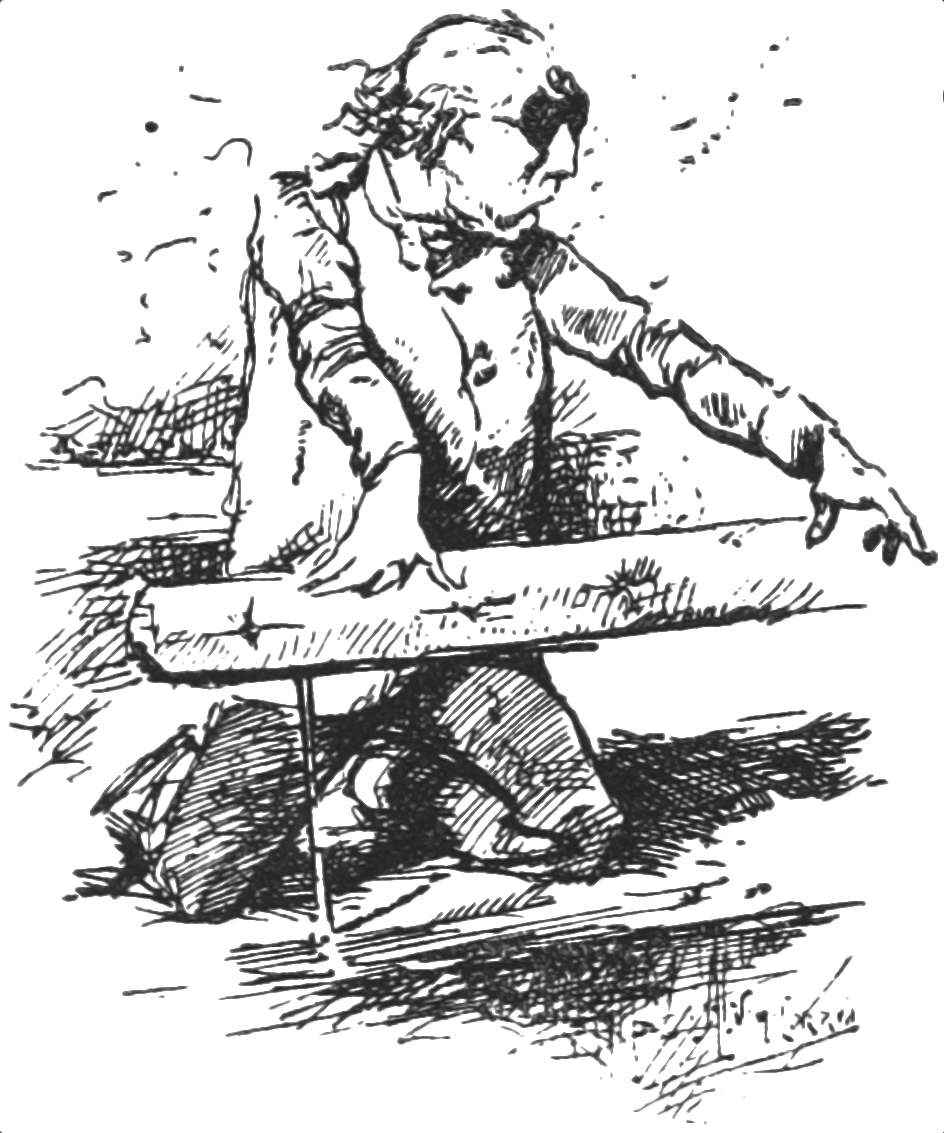
\includegraphics[width=0.5\textwidth]{16someguy}
\end{wrapfigure}

My brother noticed a pale grey smoke or haze rising among the houses in front of them, and veiling the white façade of a terrace beyond the road that appeared between the backs of the villas. Mrs~Elphinstone suddenly cried out at a number of tongues of smoky red flame leaping up above the houses in front of them against the hot, blue sky. The tumultuous noise resolved itself now into the disorderly mingling of many voices, the gride of many wheels, the creaking of waggons, and the staccato of hoofs. The lane came round sharply not fifty yards from the crossroads.

»Good heavens!« cried Mrs~Elphinstone. »What is this you are driving us into?«

My brother stopped.

For the main road was a boiling stream of people, a torrent of human beings rushing northward, one pressing on another. A great bank of dust, white and luminous in the blaze of the sun, made everything within twenty feet of the ground grey and indistinct and was perpetually renewed by the hurrying feet of a dense crowd of horses and of men and women on foot, and by the wheels of vehicles of every description.

»Way!« my brother heard voices crying. »Make way!«

It was like riding into the smoke of a fire to approach the meeting point of the lane and road; the crowd roared like a fire, and the dust was hot and pungent. And, indeed, a little way up the road a villa was burning and sending rolling masses of black smoke across the road to add to the confusion.

Two men came past them. Then a dirty woman, carrying a heavy bundle and weeping. A lost retriever dog, with hanging tongue, circled dubiously round them, scared and wretched, and fled at my brother's threat.

So much as they could see of the road Londonward between the houses to the right was a tumultuous stream of dirty, hurrying people, pent in between the villas on either side; the black heads, the crowded forms, grew into distinctness as they rushed towards the corner, hurried past, and merged their individuality again in a receding multitude that was swallowed up at last in a cloud of dust.

»Go on! Go on!« cried the voices. »Way! Way!«

One man's hands pressed on the back of another. My brother stood at the pony's head. Irresistibly attracted, he advanced slowly, pace by pace, down the lane.

Edgware had been a scene of confusion, Chalk Farm a riotous tumult, but this was a whole population in movement. It is hard to imagine that host. It had no character of its own. The figures poured out past the corner, and receded with their backs to the group in the lane. Along the margin came those who were on foot threatened by the wheels, stumbling in the ditches, blundering into one another.

The carts and carriages crowded close upon one another, making little way for those swifter and more impatient vehicles that darted forward every now and then when an opportunity showed itself of doing so, sending the people scattering against the fences and gates of the villas.

»Push on!« was the cry. »Push on! They are coming!«



In one cart stood a blind man in the uniform of the Salvation Army, gesticulating with his crooked fingers and bawling, »Eternity! Eternity!« His voice was hoarse and very loud so that my brother could hear him long after he was lost to sight in the dust. Some of the people who crowded in the carts whipped stupidly at their horses and quarrelled with other drivers; some sat motionless, staring at nothing with miserable eyes; some gnawed their hands with thirst, or lay prostrate in the bottoms of their conveyances. The horses' bits were covered with foam, their eyes bloodshot.

There were cabs, carriages, shop-carts, waggons, beyond counting; a mail cart, a road-cleaner's cart marked »Vestry of St~Pancras,« a huge timber waggon crowded with roughs. A brewer's dray rumbled by with its two near wheels splashed with fresh blood.

»Clear the way!« cried the voices. »Clear the way!«

»Eter-nity! Eter-nity!« came echoing down the road.

There were sad, haggard women tramping by, well dressed, with children that cried and stumbled, their dainty clothes smothered in dust, their weary faces smeared with tears. With many of these came men, sometimes helpful, sometimes lowering and savage. Fighting side by side with them pushed some weary street outcast in faded black rags, wide-eyed, loud-voiced, and foul-mouthed. There were sturdy workmen thrusting their way along, wretched, unkempt men, clothed like clerks or shopmen, struggling spasmodically; a wounded soldier my brother noticed, men dressed in the clothes of railway porters, one wretched creature in a nightshirt with a coat thrown over it.

\begin{wrapfigure}{O}{0.5\textwidth}
\centering
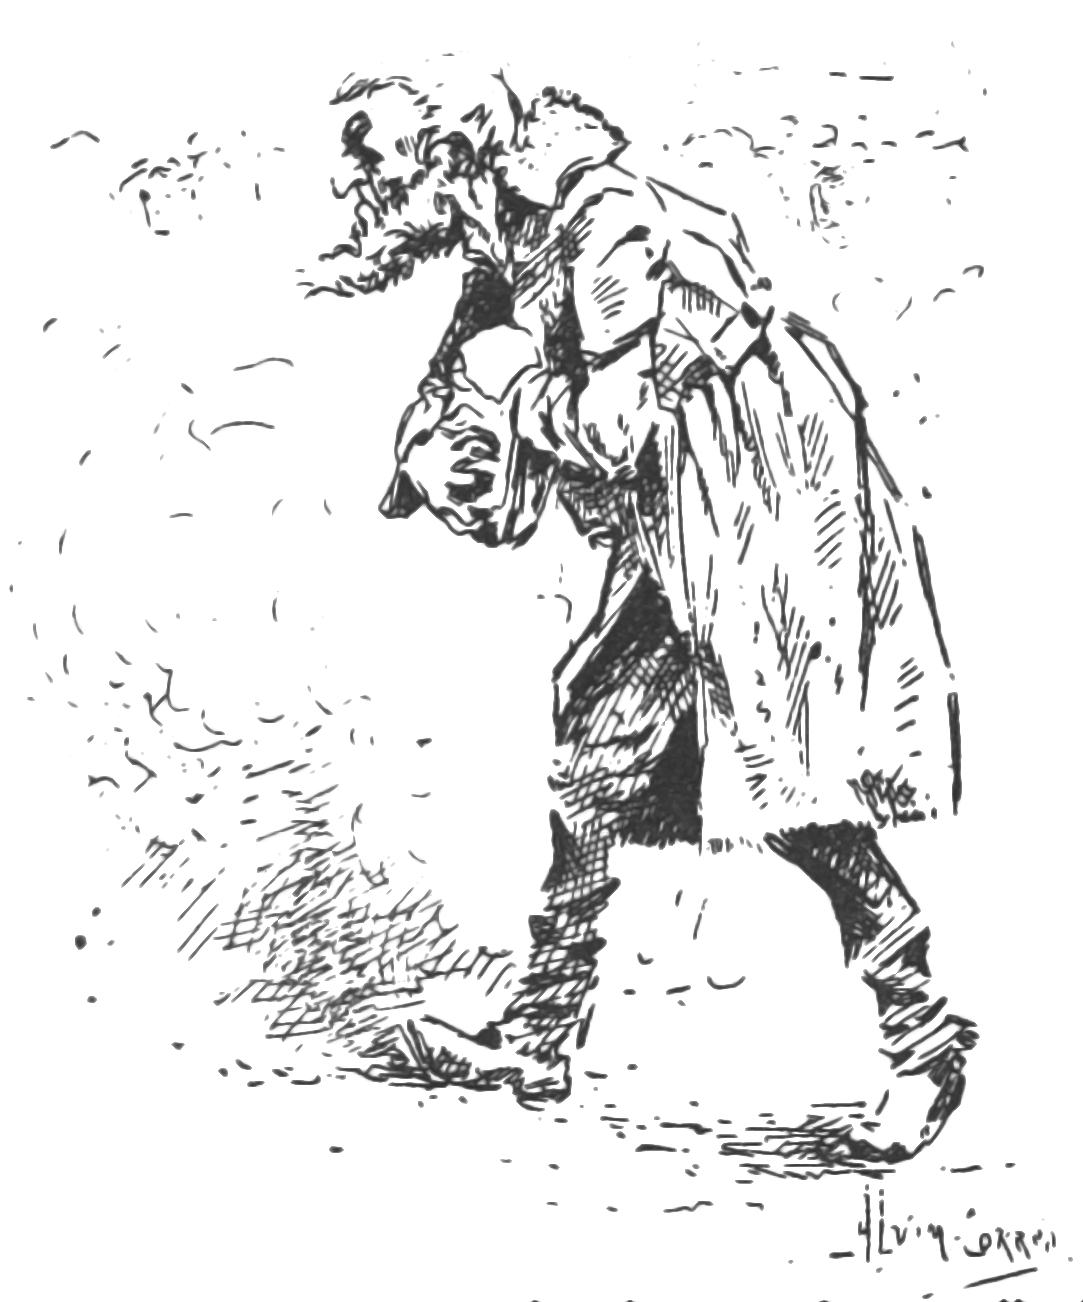
\includegraphics[width=0.5\textwidth]{16oldguy}
\end{wrapfigure}

But varied as its composition was, certain things all that host had in common. There were fear and pain on their faces, and fear behind them. A tumult up the road, a quarrel for a place in a waggon, sent the whole host of them quickening their pace; even a man so scared and broken that his knees bent under him was galvanised for a moment into renewed activity. The heat and dust had already been at work upon this multitude. Their skins were dry, their lips black and cracked. They were all thirsty, weary, and footsore. And amid the various cries one heard disputes, reproaches, groans of weariness and fatigue; the voices of most of them were hoarse and weak. Through it all ran a refrain:

»Way! Way! The Martians are coming!«

Few stopped and came aside from that flood. The lane opened slantingly into the main road with a narrow opening, and had a delusive appearance of coming from the direction of London. Yet a kind of eddy of people drove into its mouth; weaklings elbowed out of the stream, who for the most part rested but a moment before plunging into it again. A little way down the lane, with two friends bending over him, lay a man with a bare leg, wrapped about with bloody rags. He was a lucky man to have friends.

A little old man, with a grey military moustache and a filthy black frock coat, limped out and sat down beside the trap, removed his boot—his sock was blood-stained—shook out a pebble, and hobbled on again; and then a little girl of eight or nine, all alone, threw herself under the hedge close by my brother, weeping.

»I can't go on! I can't go on!«

My brother woke from his torpor of astonishment and lifted her up, speaking gently to her, and carried her to Miss Elphinstone. So soon as my brother touched her she became quite still, as if frightened.

»Ellen!« shrieked a woman in the crowd, with tears in her voice—»Ellen!« And the child suddenly darted away from my brother, crying »Mother!«

»They are coming,« said a man on horseback, riding past along the lane.

»Out of the way, there!« bawled a coachman, towering high; and my brother saw a closed carriage turning into the lane.

The people crushed back on one another to avoid the horse. My brother pushed the pony and chaise back into the hedge, and the man drove by and stopped at the turn of the way. It was a carriage, with a pole for a pair of horses, but only one was in the traces. My brother saw dimly through the dust that two men lifted out something on a white stretcher and put it gently on the grass beneath the privet hedge.

One of the men came running to my brother.

»Where is there any water?« he said. »He is dying fast, and very thirsty. It is Lord Garrick.«

»Lord Garrick!« said my brother; »the Chief Justice?«

»The water?« he said.

»There may be a tap,« said my brother, »in some of the houses. We have no water. I dare not leave my people.«

The man pushed against the crowd towards the gate of the corner house.

»Go on!« said the people, thrusting at him. »They are coming! Go on!«

Then my brother's attention was distracted by a bearded, eagle-faced man lugging a small handbag, which split even as my brother's eyes rested on it and disgorged a mass of sovereigns that seemed to break up into separate coins as it struck the ground. They rolled hither and thither among the struggling feet of men and horses. The man stopped and looked stupidly at the heap, and the shaft of a cab struck his shoulder and sent him reeling. He gave a shriek and dodged back, and a cartwheel shaved him narrowly.

»Way!« cried the men all about him. »Make way!«

So soon as the cab had passed, he flung himself, with both hands open, upon the heap of coins, and began thrusting handfuls in his pocket. A horse rose close upon him, and in another moment, half rising, he had been borne down under the horse's hoofs.

»Stop!« screamed my brother, and pushing a woman out of his way, tried to clutch the bit of the horse.

Before he could get to it, he heard a scream under the wheels, and saw through the dust the rim passing over the poor wretch's back. The driver of the cart slashed his whip at my brother, who ran round behind the cart. The multitudinous shouting confused his ears. The man was writhing in the dust among his scattered money, unable to rise, for the wheel had broken his back, and his lower limbs lay limp and dead. My brother stood up and yelled at the next driver, and a man on a black horse came to his assistance.

»Get him out of the road,« said he; and, clutching the man's collar with his free hand, my brother lugged him sideways. But he still clutched after his money, and regarded my brother fiercely, hammering at his arm with a handful of gold. »Go on! Go on!« shouted angry voices behind. »Way! Way!«

\begin{letter}
	\begin{wrapfigure}{O}{0.5\textwidth}
		\centering
		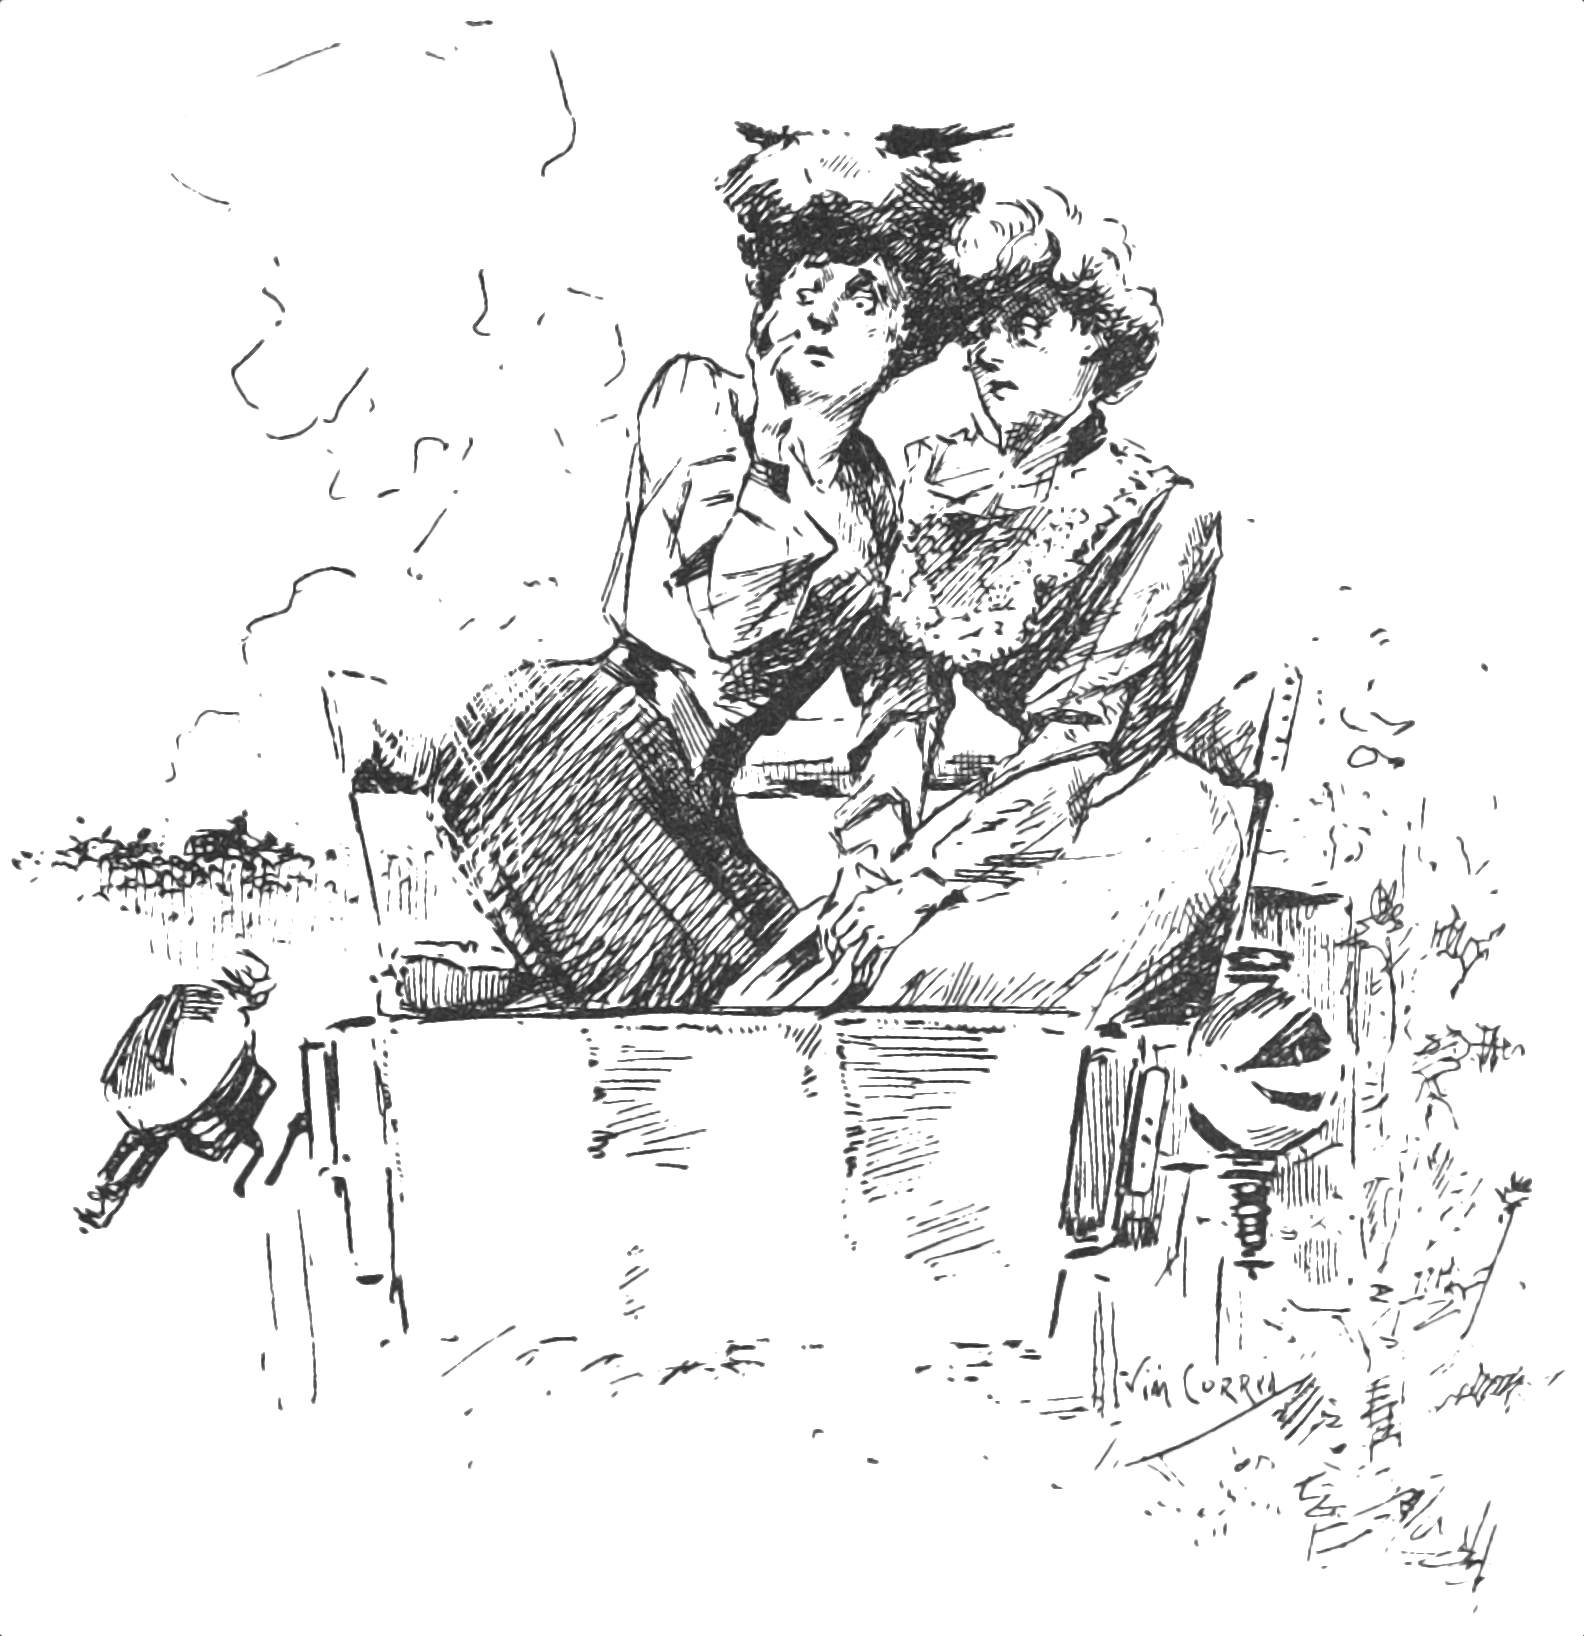
\includegraphics[width=0.5\textwidth]{16twowomen}
	\end{wrapfigure}
\end{letter}

There was a smash as the pole of a carriage crashed into the cart that the man on horseback stopped. My brother looked up, and the man with the gold twisted his head round and bit the wrist that held his collar. There was a concussion, and the black horse came staggering sideways, and the carthorse pushed beside it. A hoof missed my brother's foot by a hair's breadth. He released his grip on the fallen man and jumped back. He saw anger change to terror on the face of the poor wretch on the ground, and in a moment he was hidden and my brother was borne backward and carried past the entrance of the lane, and had to fight hard in the torrent to recover it.



He saw Miss Elphinstone covering her eyes, and a little child, with all a child's want of sympathetic imagination, staring with dilated eyes at a dusty something that lay black and still, ground and crushed under the rolling wheels. »Let us go back!« he shouted, and began turning the pony round. »We cannot cross this—hell,« he said and they went back a hundred yards the way they had come, until the fighting crowd was hidden. As they passed the bend in the lane my brother saw the face of the dying man in the ditch under the privet, deadly white and drawn, and shining with perspiration. The two women sat silent, crouching in their seat and shivering.

Then beyond the bend my brother stopped again. Miss Elphinstone was white and pale, and her sister-in-law sat weeping, too wretched even to call upon »George.« My brother was horrified and perplexed. So soon as they had retreated he realised how urgent and unavoidable it was to attempt this crossing. He turned to Miss Elphinstone, suddenly resolute.

»We must go that way,« he said, and led the pony round again.

\begin{a4}
	\begin{wrapfigure}{O}{0.5\textwidth}
		\centering
		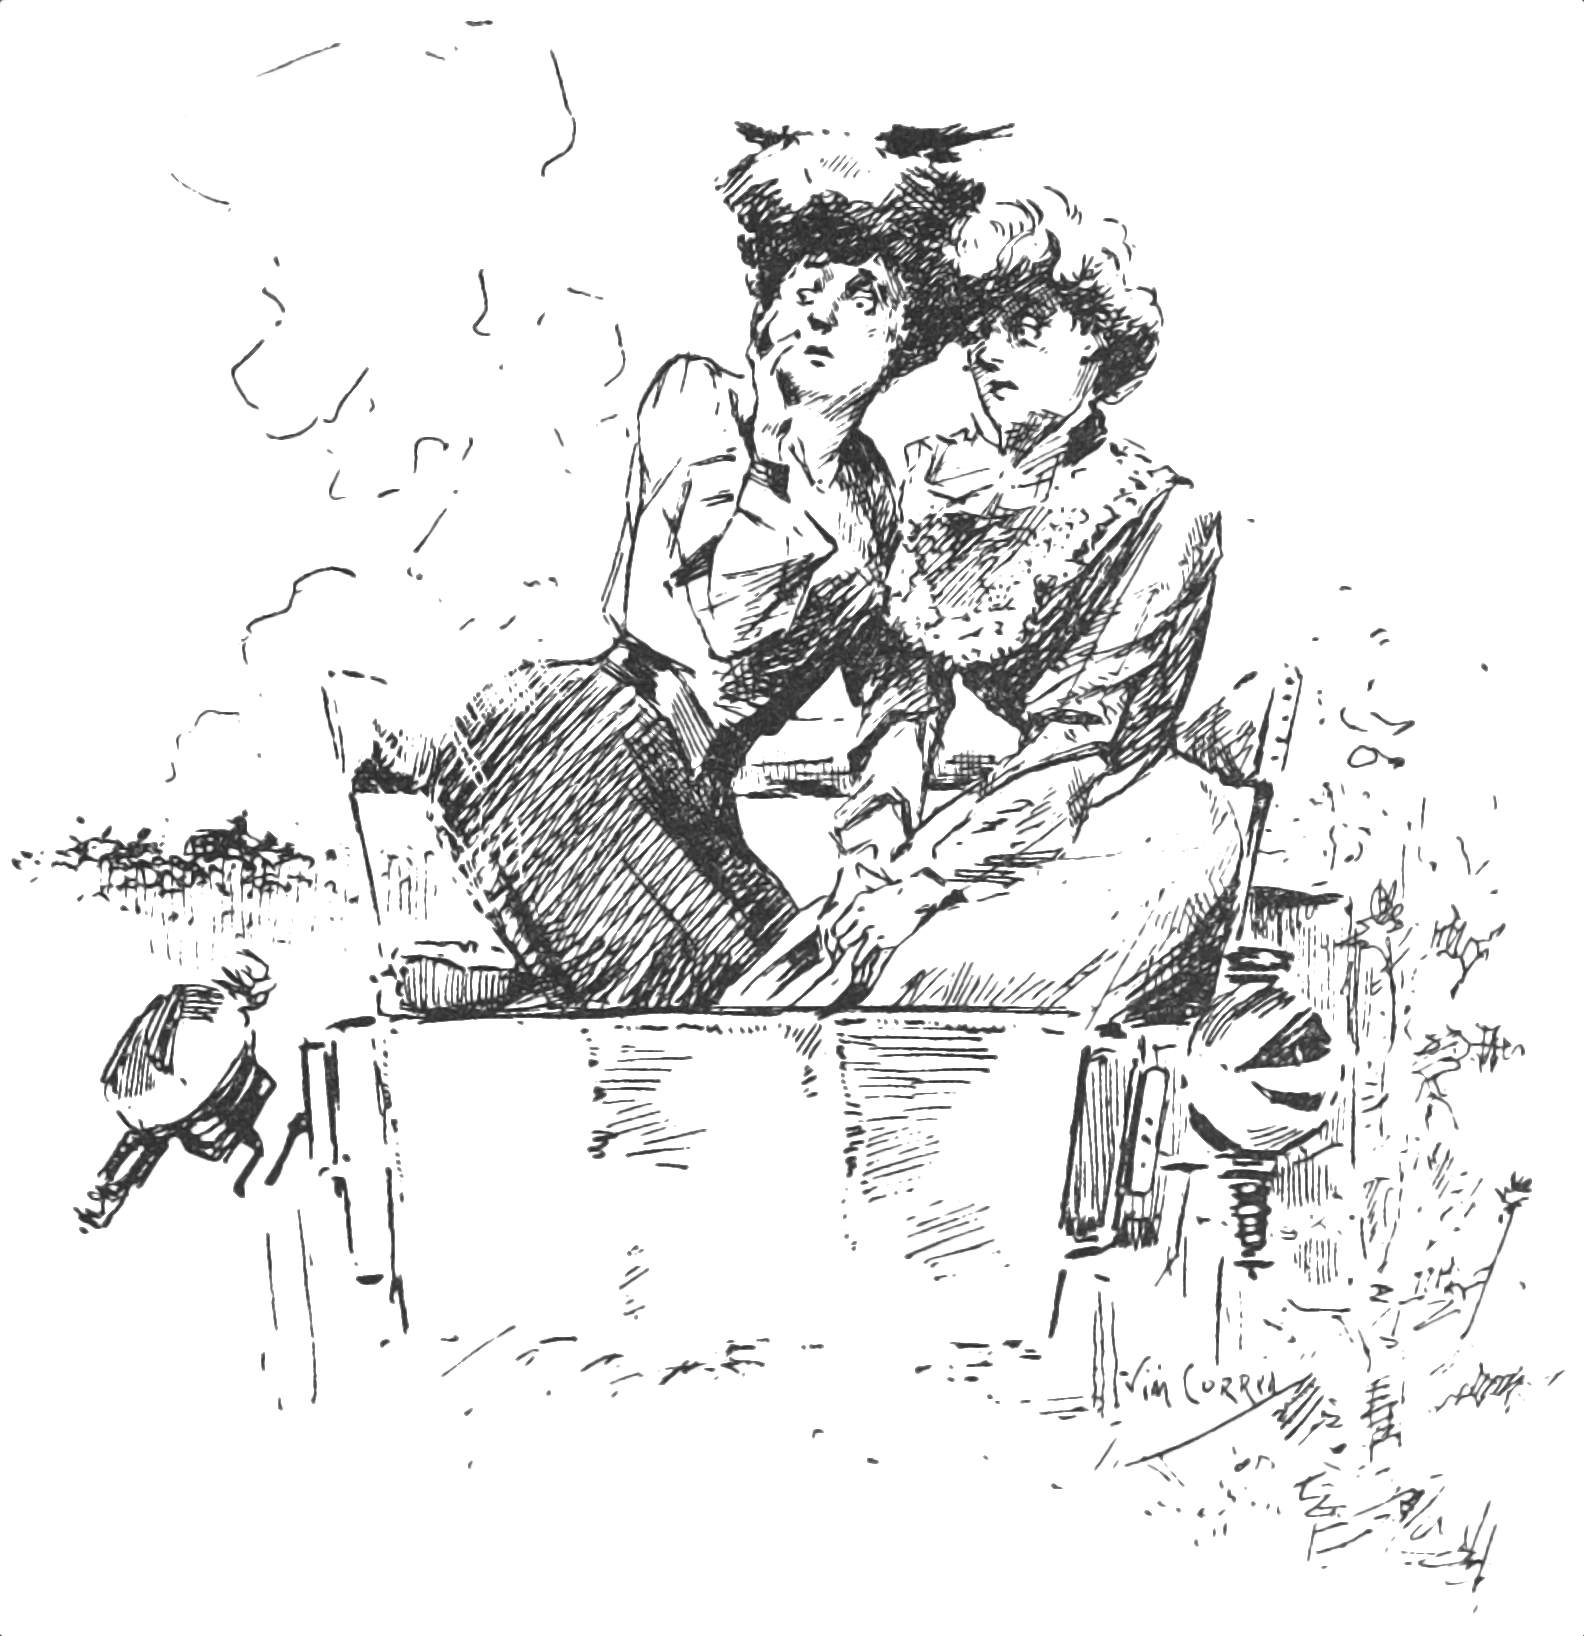
\includegraphics[width=0.5\textwidth]{16twowomen}
	\end{wrapfigure}
\end{a4}

For the second time that day this girl proved her quality. To force their way into the torrent of people, my brother plunged into the traffic and held back a cab horse, while she drove the pony across its head. A waggon locked wheels for a moment and ripped a long splinter from the chaise. In another moment they were caught and swept forward by the stream. My brother, with the cabman's whip marks red across his face and hands, scrambled into the chaise and took the reins from her.

»Point the revolver at the man behind,« he said, giving it to her, »if he presses us too hard. No!—point it at his horse.«

Then he began to look out for a chance of edging to the right across the road. But once in the stream he seemed to lose volition, to become a part of that dusty rout. They swept through Chipping Barnet with the torrent; they were nearly a mile beyond the centre of the town before they had fought across to the opposite side of the way. It was din and confusion indescribable; but in and beyond the town the road forks repeatedly, and this to some extent relieved the stress.

They struck eastward through Hadley, and there on either side of the road, and at another place farther on they came upon a great multitude of people drinking at the stream, some fighting to come at the water. And farther on, from a lull near East Barnet, they saw two trains running slowly one after the other without signal or order—trains swarming with people, with men even among the coals behind the engines—going northward along the Great Northern Railway. My brother supposes they must have filled outside London, for at that time the furious terror of the people had rendered the central termini impossible.

Near this place they halted for the rest of the afternoon, for the violence of the day had already utterly exhausted all three of them. They began to suffer the beginnings of hunger; the night was cold, and none of them dared to sleep. And in the evening many people came hurrying along the road nearby their stopping place, fleeing from unknown dangers before them, and going in the direction from which my brother had come.

\begin{a4}
	\begin{figure}[b!]
		\centering
		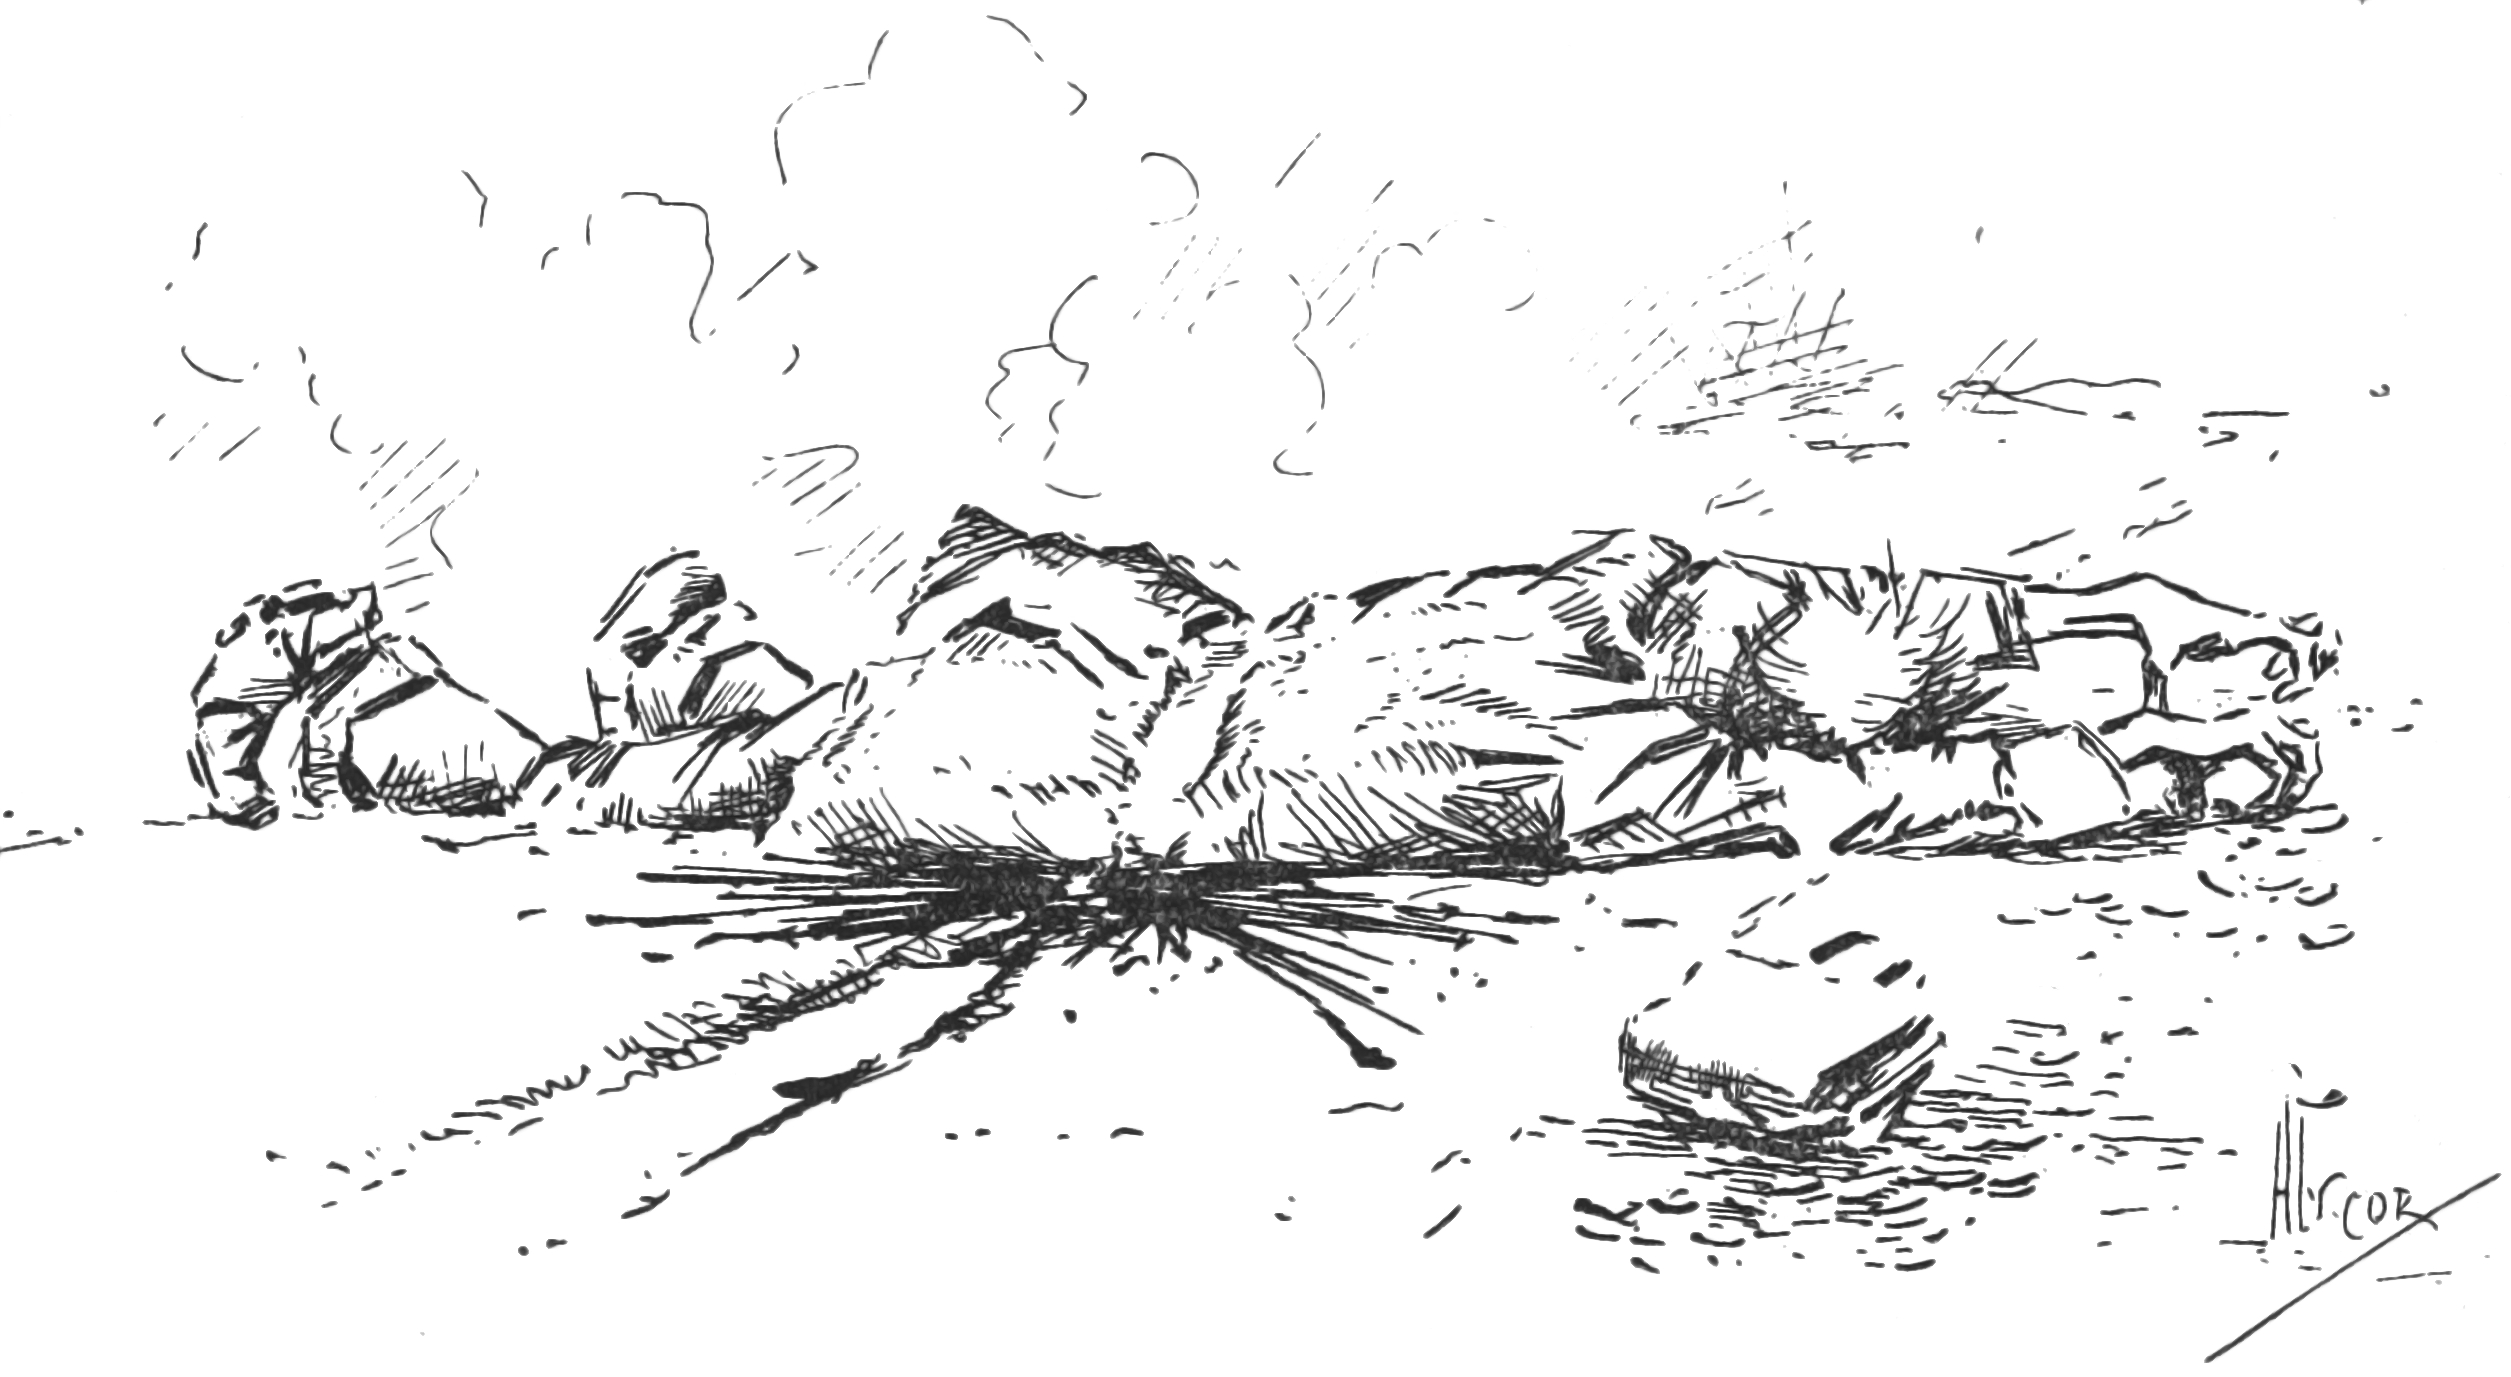
\includegraphics[width=\textwidth]{16tailpiece}
	\end{figure}
\end{a4}

\begin{letter}
	\begin{figure}[b!]
		\centering
		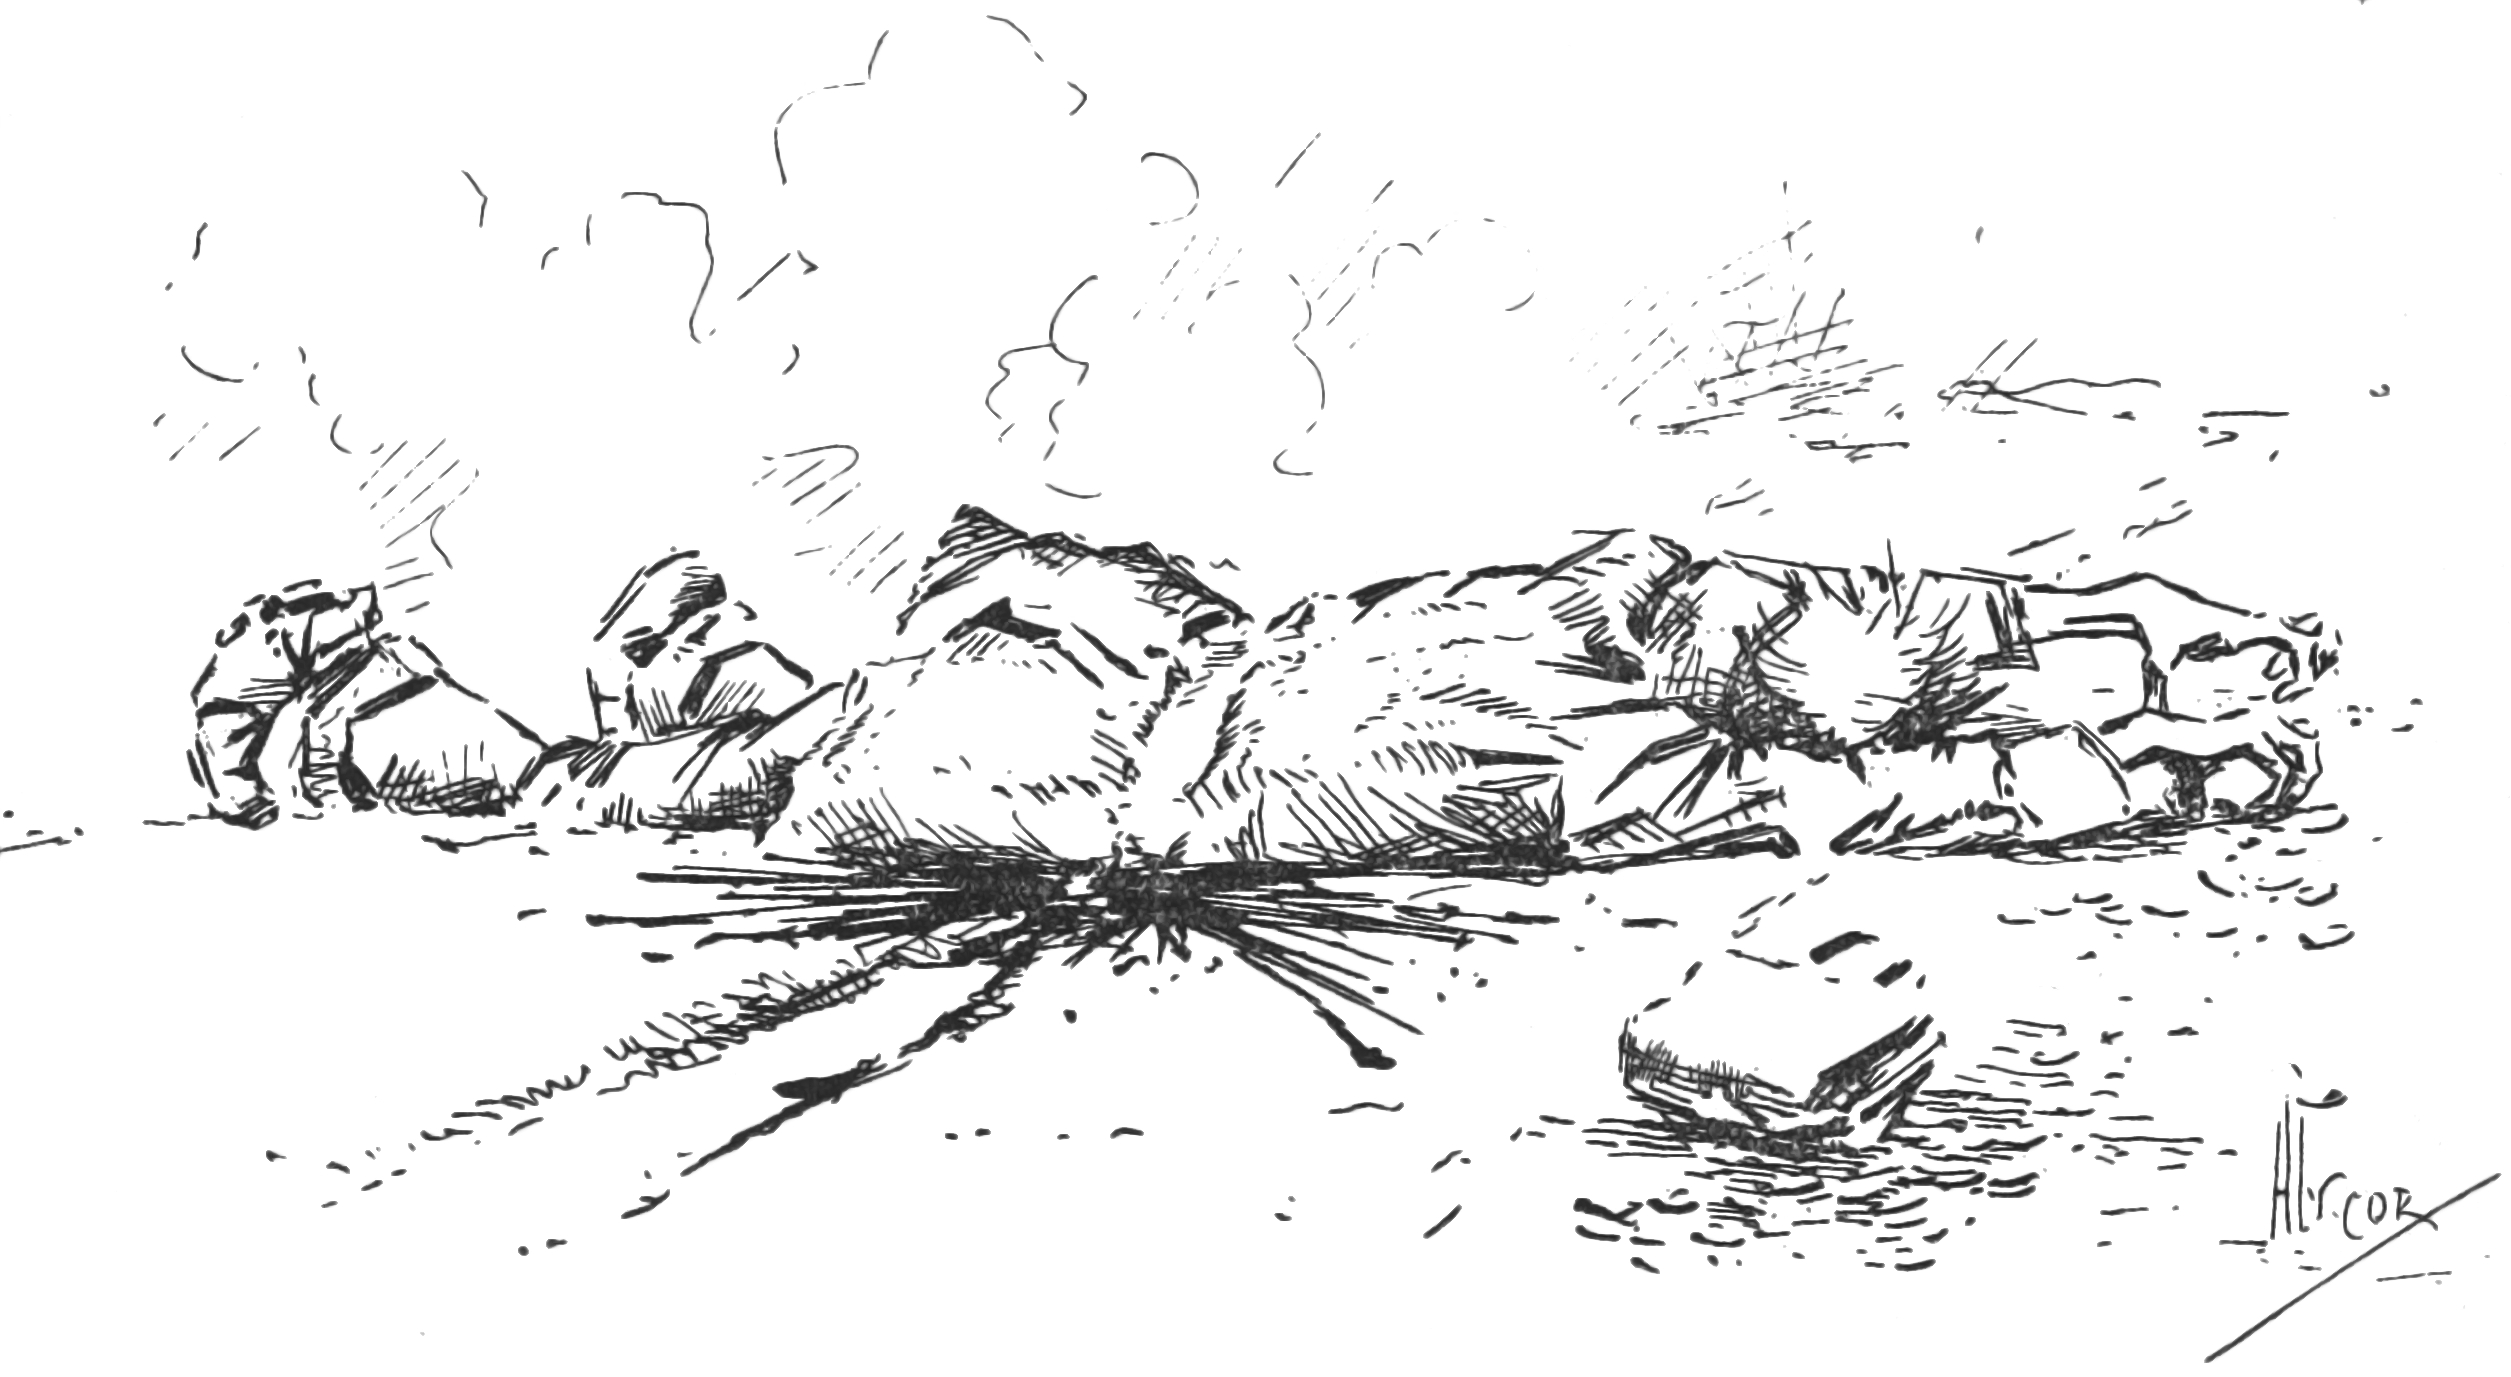
\includegraphics[width=.7\textwidth]{16tailpiece}
	\end{figure}
\end{letter}
